\documentclass[a4paper, 12pt]{article}
\usepackage[UTF8]{ctex}
\usepackage{xcolor}  % 导入 xcolor 包
\usepackage{color}
\usepackage{fancyhdr}  % 引入 fancyhdr 宏包
\usepackage{lipsum}    % 用于生成示例文本
\usepackage{graphicx}		%用于引用图片的包
\usepackage{amsmath}

% 定义浅灰色
\definecolor{lightgray}{RGB}{211,211,211}

\pagestyle{fancy}      % 使用 fancyhdr 提供的页面样式

\fancyhf             % 清除默认设置

\fancyfoot[R]{\thepage} % 将页码放在右下角

\begin{document}

  \title{系统开发工具基础第一次实验报告}
  \author{姓名:杨子程\ 学号:23020007145\ 专业:计算机科学与技术}
  \date{\today}
  \maketitle

  \tableofcontents
  \newpage

  \section{关于Git的使用}
  \subsection{创建一个可使用Git的本地仓库}

首先,在本地的一个合适的目录下新建一个用于作为仓库的文件夹。然后,使用Git Bash切换到对应的文件夹,使用命令

\colorbox{lightgray}{\texttt{git init}}

相关过程:

\begin{figure}[h]
  \centering
  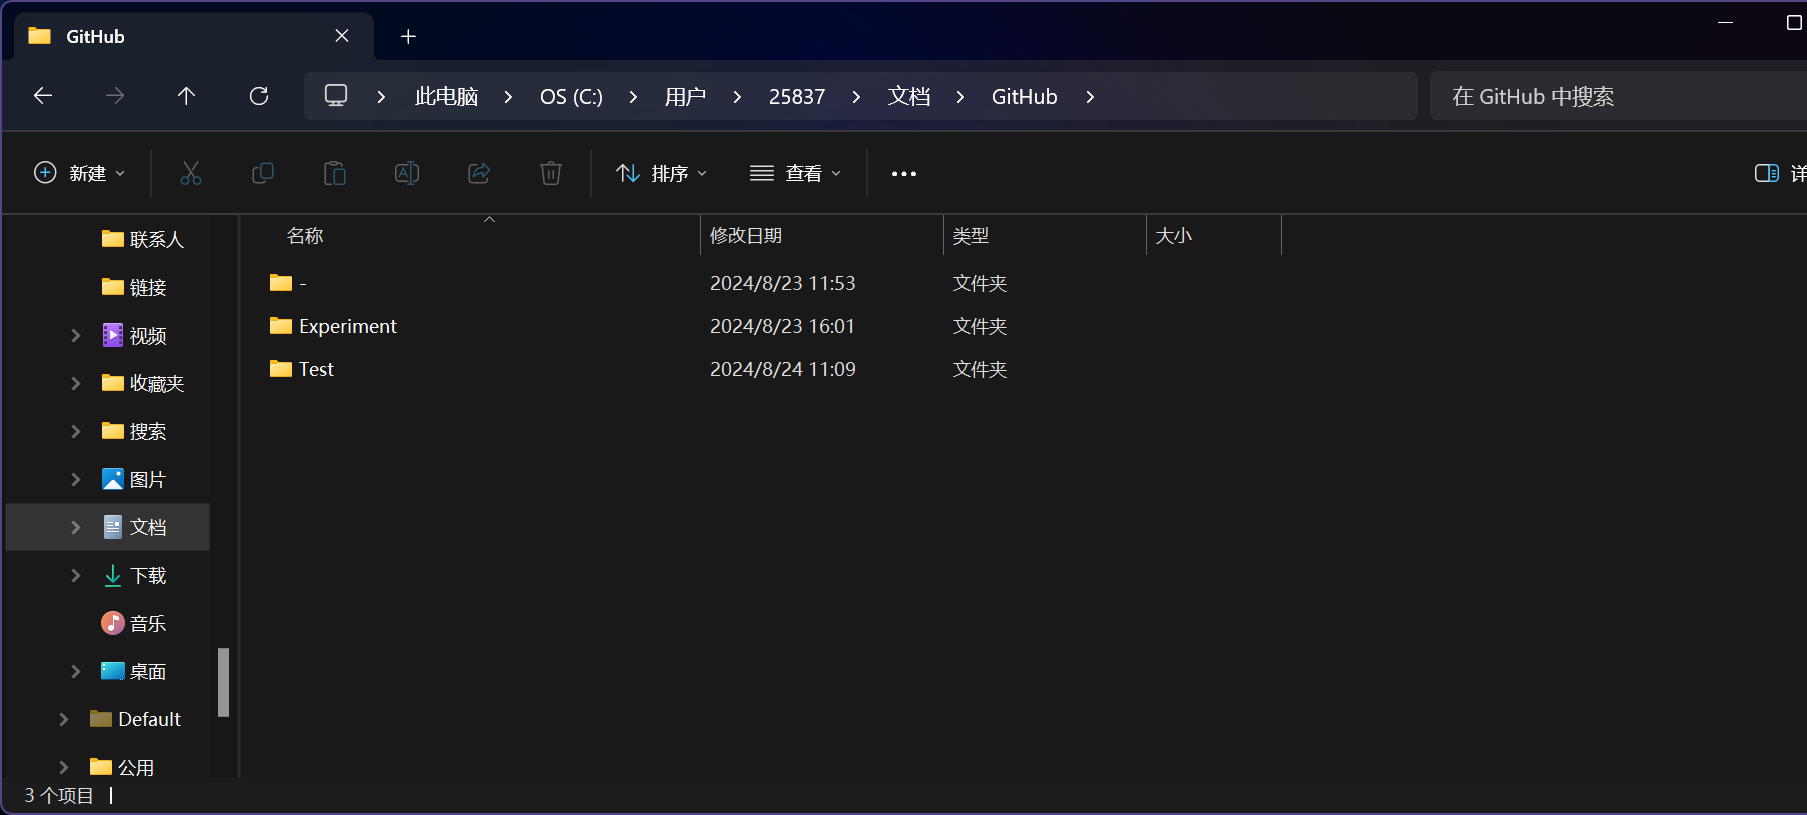
\includegraphics[width=1\textwidth]{im1}
  \caption{本地文件夹}
  \label{image-myimage}
\end{figure}

\begin{figure}[h]
  \centering
  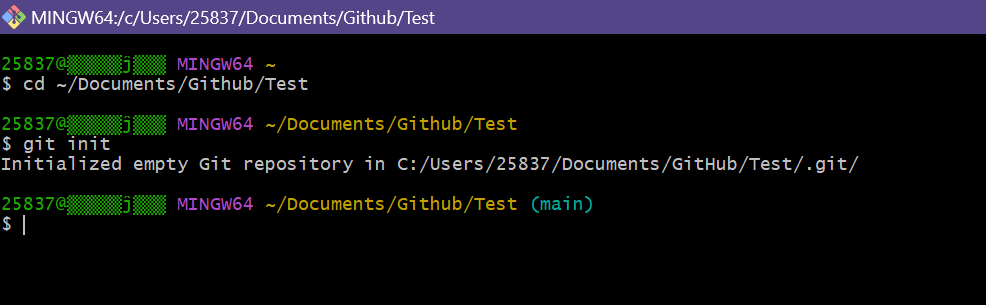
\includegraphics[width=1\textwidth]{im2}
  \caption{Git Bash的操作}
  \label{image-myimage}
\end{figure}

\begin{figure}[h]
  \centering
  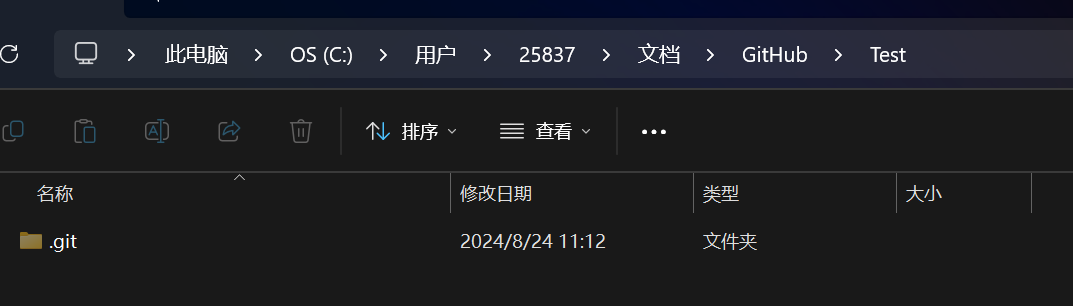
\includegraphics[width=1\textwidth]{im3}
  \caption{完成创建}
  \label{image-myimage}
\end{figure}

\clearpage

  \subsection{将本地仓库和Github作链接}

首先,登录到Github创建一个新的Repository,用来作为储存你新项目的云端仓库,之后使用Git Bash切换到你的本地仓库,使用命令进行链接操作。命令如下:

\colorbox{lightgray}{\texttt{git remote add origin 你的Github上对应的Repository的网址}}

相关过程:

\begin{figure}[h]
  \centering
  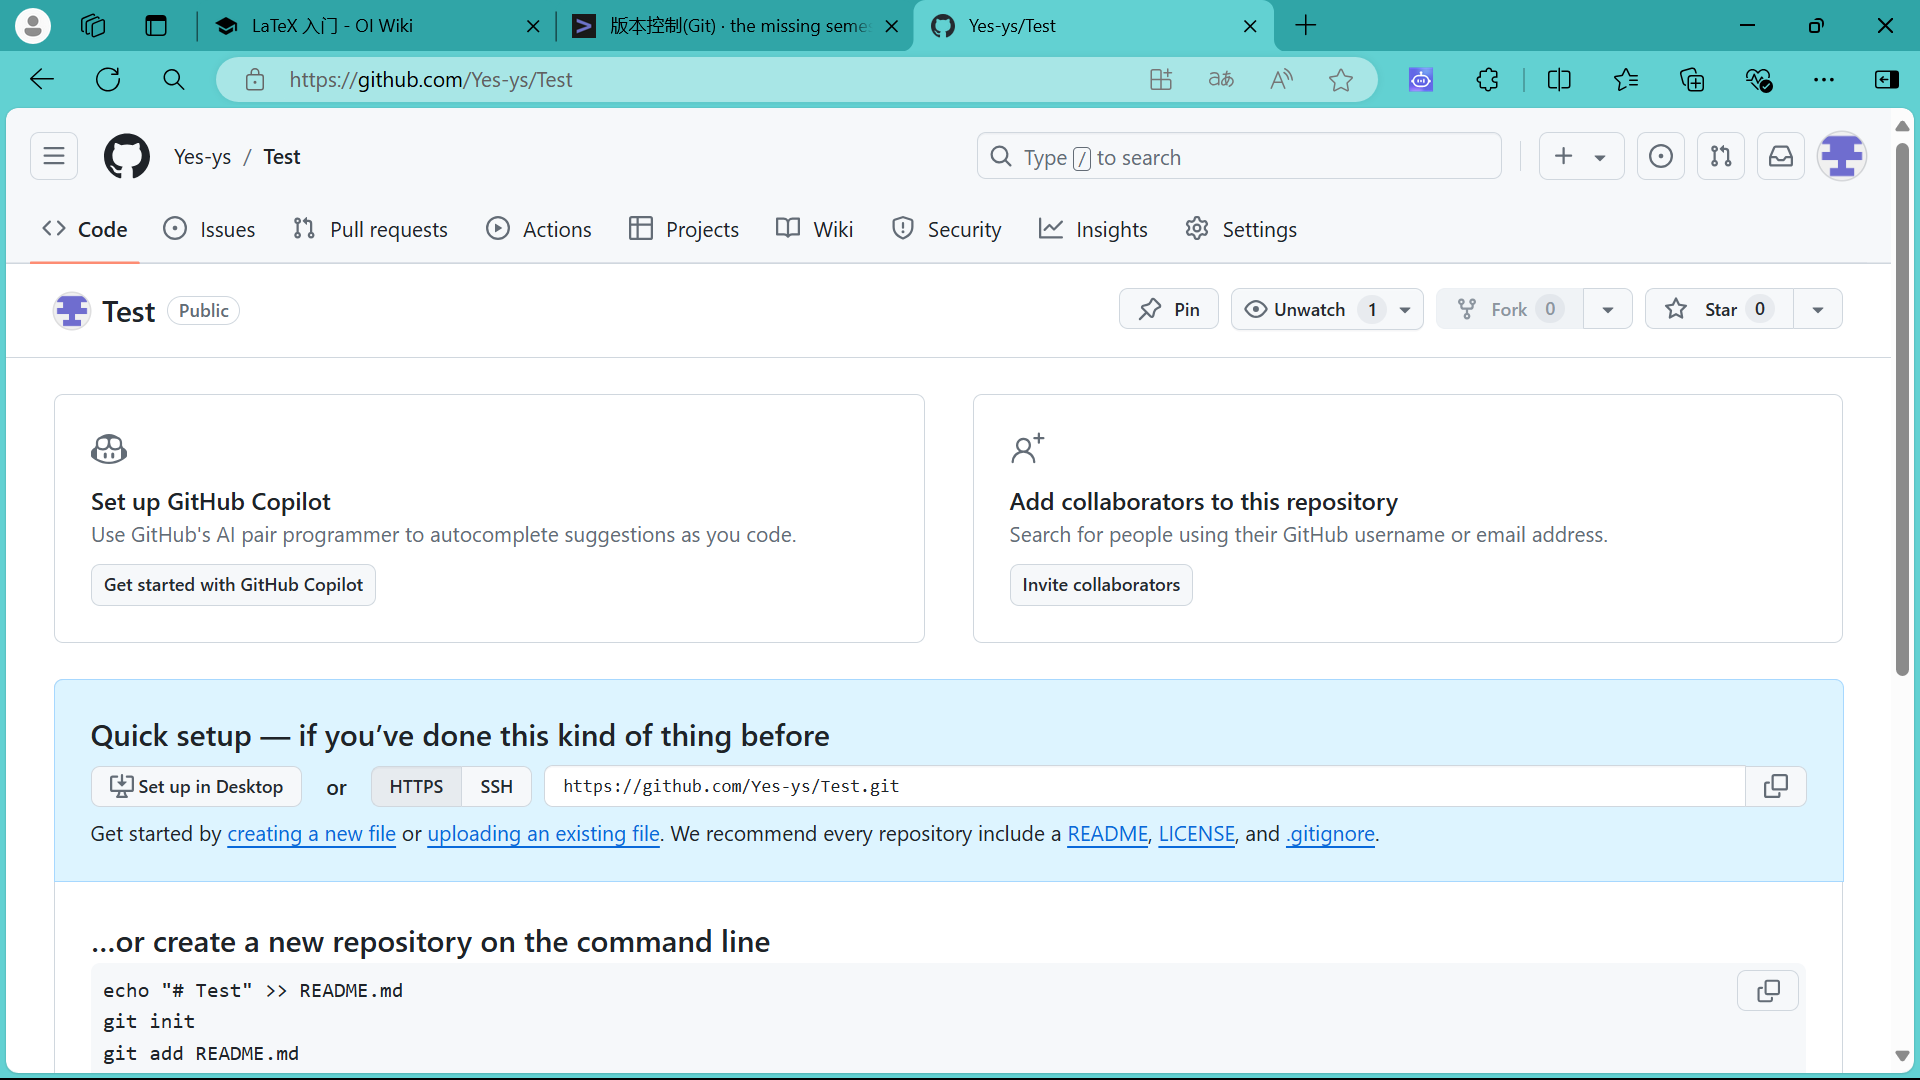
\includegraphics[width=1\textwidth]{im5}
  \caption{Github上的操作}
  \label{image-myimage}
\end{figure}

\begin{figure}[h]
  \centering
  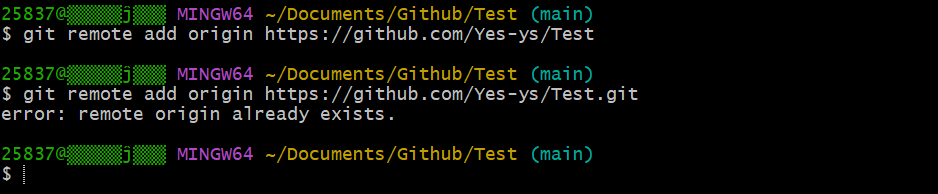
\includegraphics[width=1\textwidth]{im4}
  \caption{Git Bash的操作(通过重复执行上述命令Git Bash返回的信息可以看出操作成功)}
  \label{image-myimage}
\end{figure}

\clearpage

  \subsection{将本地文件添加到Github仓库中}

首先,对本地文件夹的内容进行更新(此处新建了一个txt文件)。然后,将工作区的更新存入暂存区。之后,对暂存区的内容进行提交。最后,上传到Github。

相关命令:

\colorbox{lightgray}{\texttt{git add .}} 将整个工作区更新的内容存入暂存区

\colorbox{lightgray}{\texttt{git commit -m"提示信息"}} 将暂存区内容提交

\colorbox{lightgray}{\texttt{git push -u origin main}} 上传到Github

相关过程:

\begin{figure}[h]
  \centering
  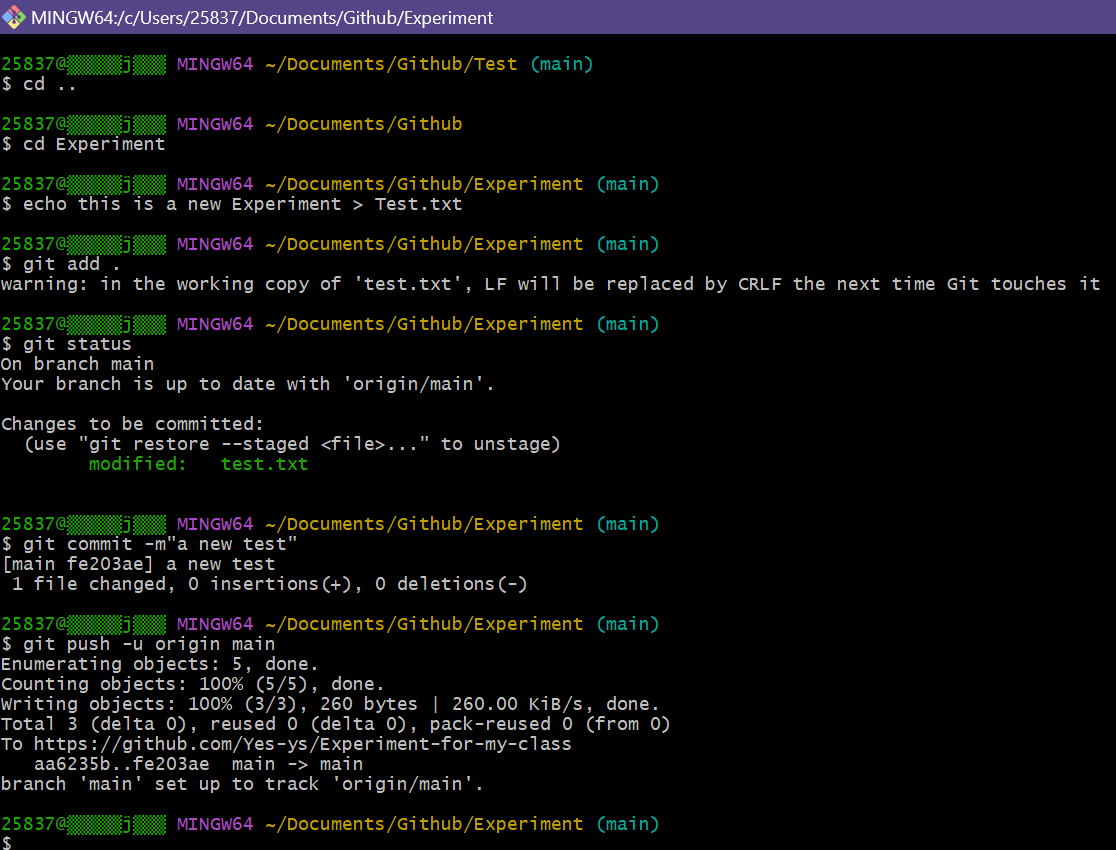
\includegraphics[scale=0.4]{im6}
  \caption{Git Bash的操作}
  \label{image-myimage}
\end{figure}

\begin{figure}[h]
  \centering
  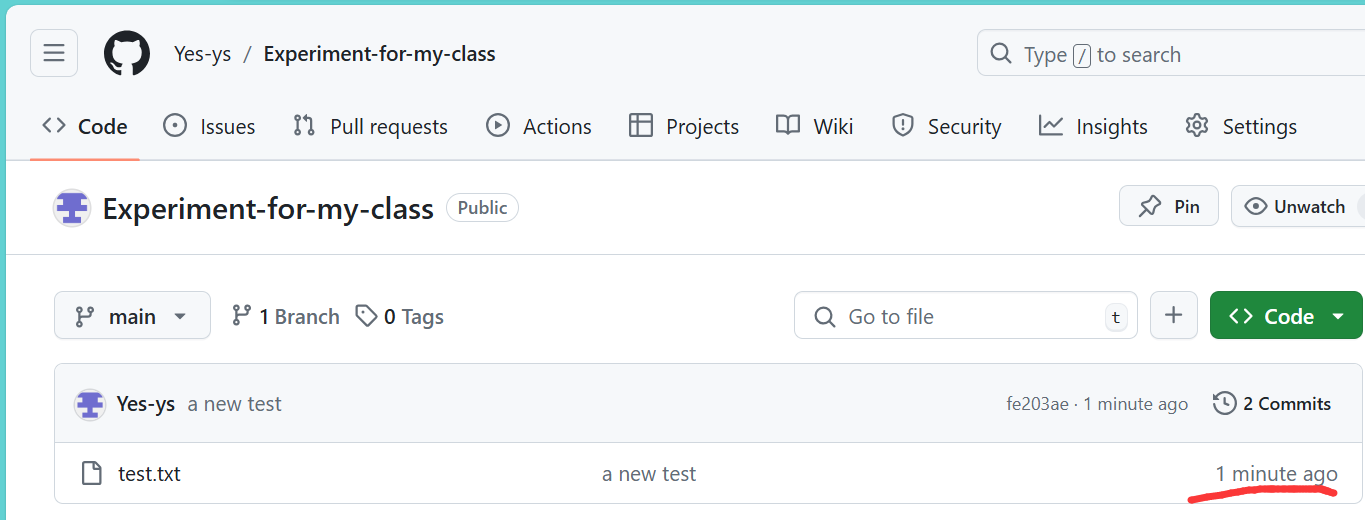
\includegraphics[scale=0.3]{im7}
  \caption{操作后的结果}
  \label{image-myimage}
\end{figure}

\clearpage  % 确保在图片页面后换页

  \subsection{创建新分支并在新分支上进行操作}

在Git Bash上进行操作,先创建一个新的分支,后以新分支在本地文件夹下新建文件,并提交。

命令如下:

\colorbox{lightgray}{\texttt{git branch new-branch}} 创建新分支,名为new-branch

\colorbox{lightgray}{\texttt{git checkout new-branch}} 将HEAD切换到new-branch

\colorbox{lightgray}{\texttt{echo this is a new-branch \textgreater\ new\_test.txt}} 新建txt文件

\colorbox{lightgray}{\texttt{git add new\_test.txt}}

\colorbox{lightgray}{\texttt{git commit -m"on new branch to test"}} 提交

\begin{figure}[h]
  \centering
  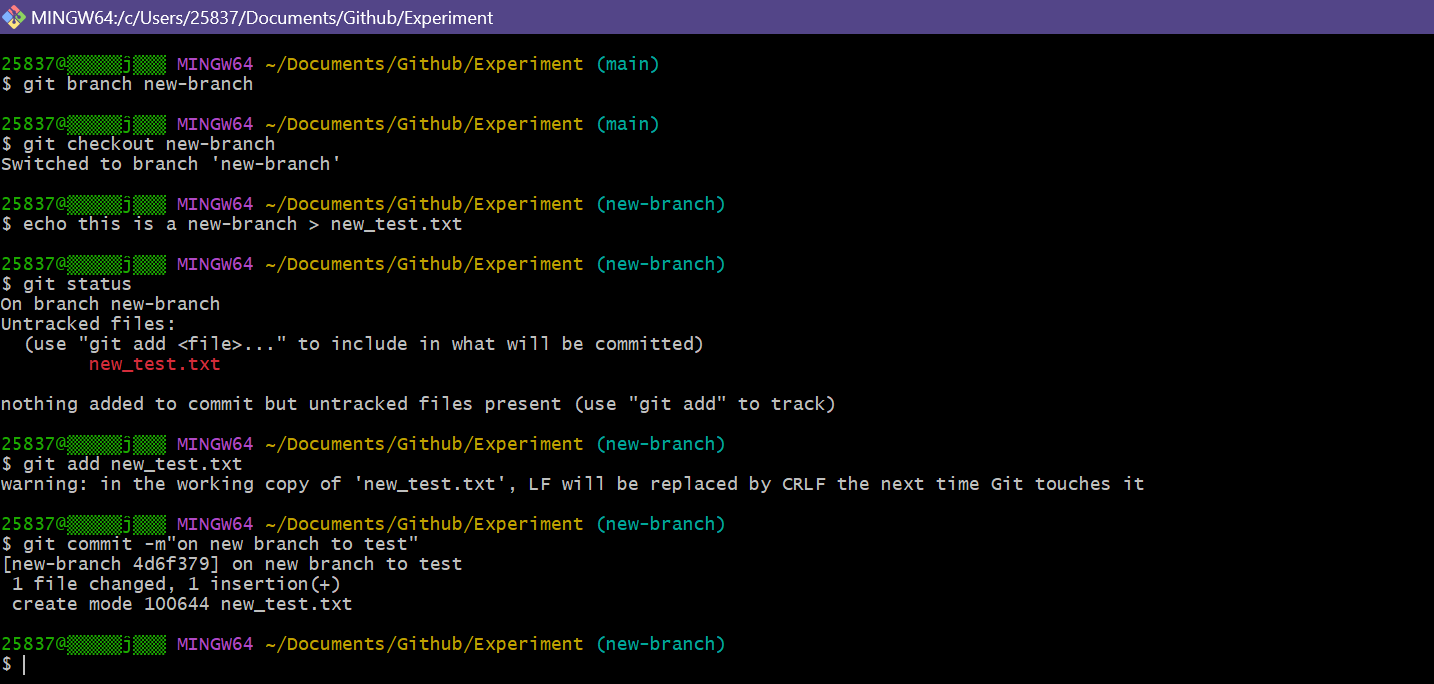
\includegraphics[width=1\textwidth]{im8}
  \caption{操作后的结果}
  \label{image-myimage}
\end{figure}

\clearpage

  \subsection{合并分支操作}

将HEAD切换回main分支,再进行合并操作,相关命令如下:

\colorbox{lightgray}{\texttt{git switch main}} 切换到main分支

\colorbox{lightgray}{\texttt{git merge new-branch}} 合并分支new-branch

\begin{figure}[h]
  \centering
  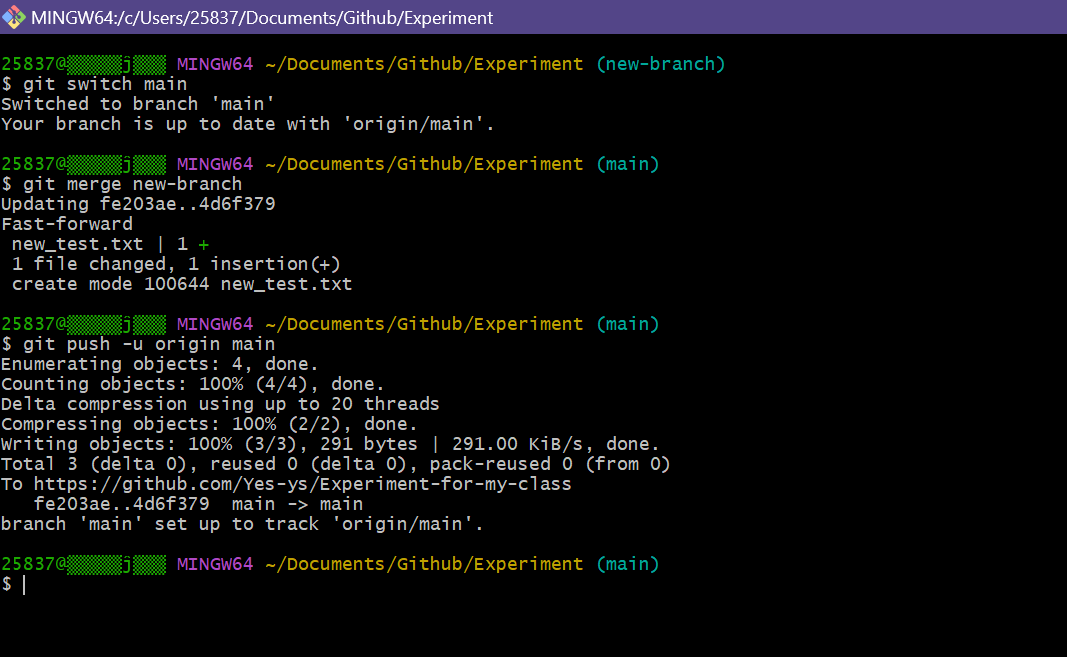
\includegraphics[width=1\textwidth]{im9}
  \caption{Git Bash上的操作}
  \label{image-myimage}
\end{figure}

\begin{figure}[h!]
  \centering
  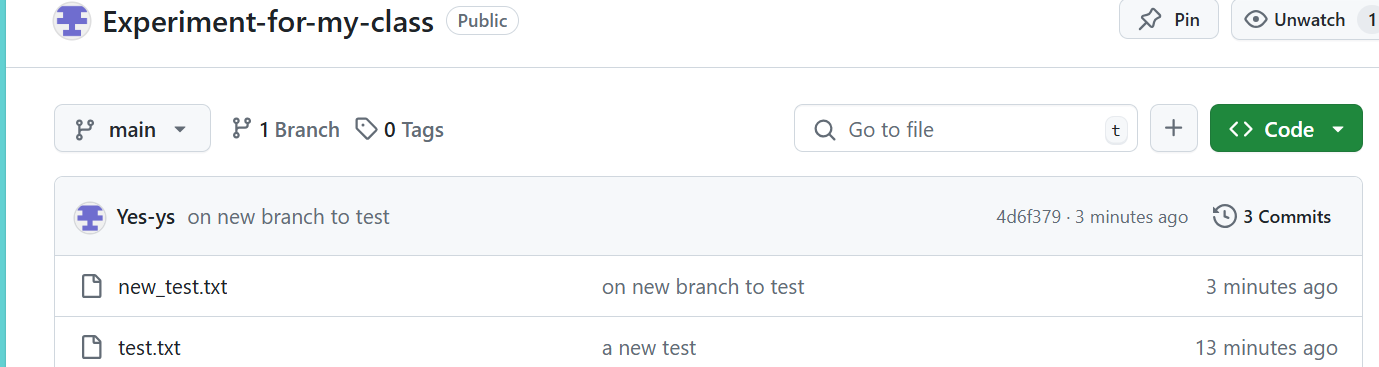
\includegraphics[width=1\textwidth]{im10}
  \caption{操作后的结果(合并后执行了上传到Github中的操作)}
  \label{image-myimage}
\end{figure}

\clearpage

  \subsection{从云端向本地的克隆操作}

切换到最开始创建的本地仓库Test,克隆Github上的Repository,再使用cat查看克隆而来的txt文件

相关命令:

\colorbox{lightgray}{\texttt{git clone Repository的网址}}

\begin{figure}[h!]
  \centering
  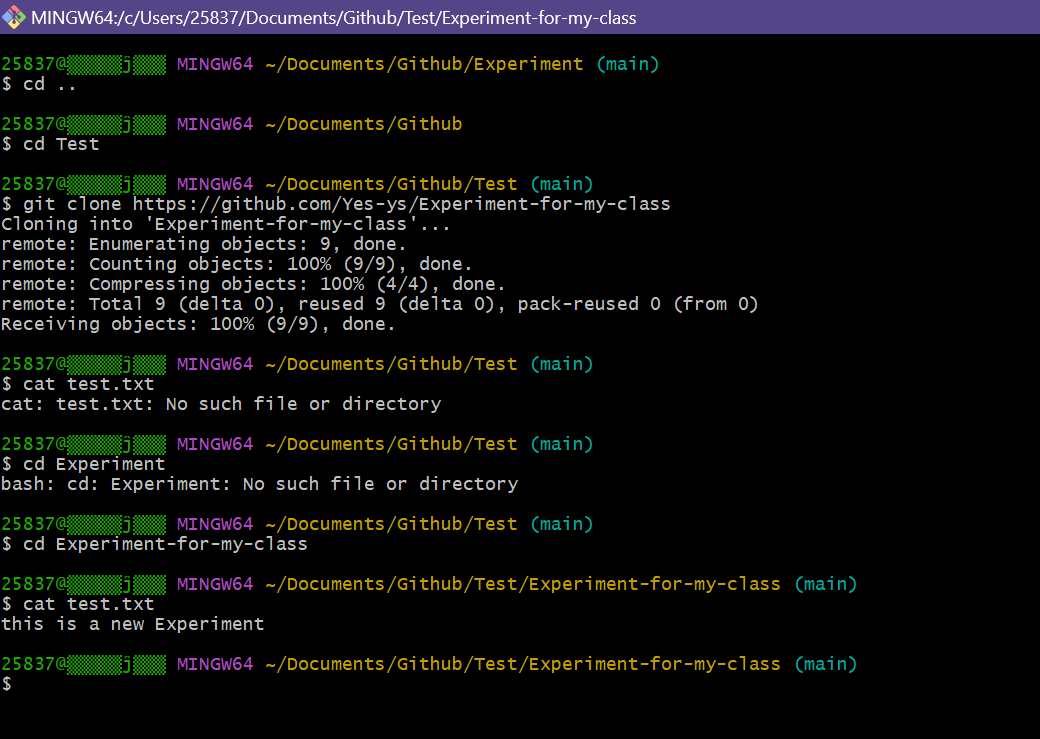
\includegraphics[width=1\textwidth]{im11}
  \caption{操作及结果}
  \label{image-myimage}
\end{figure}

\clearpage

  \subsection{撤销对工作区文件的修改}

切换回一般做实验用的本地仓库Experiment,对test文件进行修改后执行撤销操作,再检查其中的内容。

相关命令:

\colorbox{lightgray}{\texttt{git checkout -- 文件名}} 撤销工作区文件的修改

\colorbox{lightgray}{\texttt{git checkout -- test.txt}}  例如这样

\begin{figure}[h!]
  \centering
  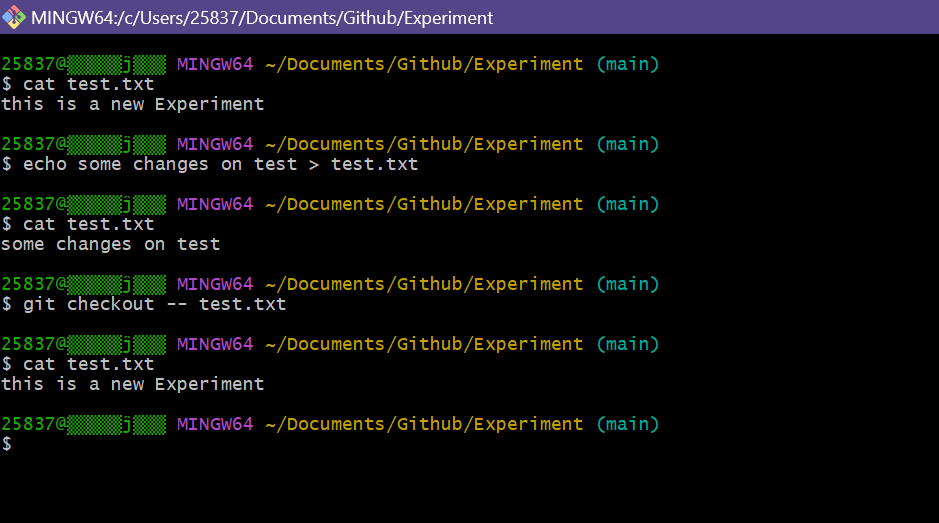
\includegraphics[width=1\textwidth]{im12}
  \caption{操作及结果}
  \label{image-myimage}
\end{figure}

\clearpage

  \subsection{撤销对缓存区的修改}

将新修改的工作区添加进入缓存区后,进行撤销操作。

相关命令:

\colorbox{lightgray}{\texttt{git reset HEAD 加入缓存区的文件名}} 撤销缓存区的修改
\colorbox{lightgray}{\texttt{git reset HEAD test.txt}} 例如这样
\colorbox{lightgray}{\texttt{git status}} 查看当前git的状态(显示实验的结果)

\begin{figure}[h!]
  \centering
  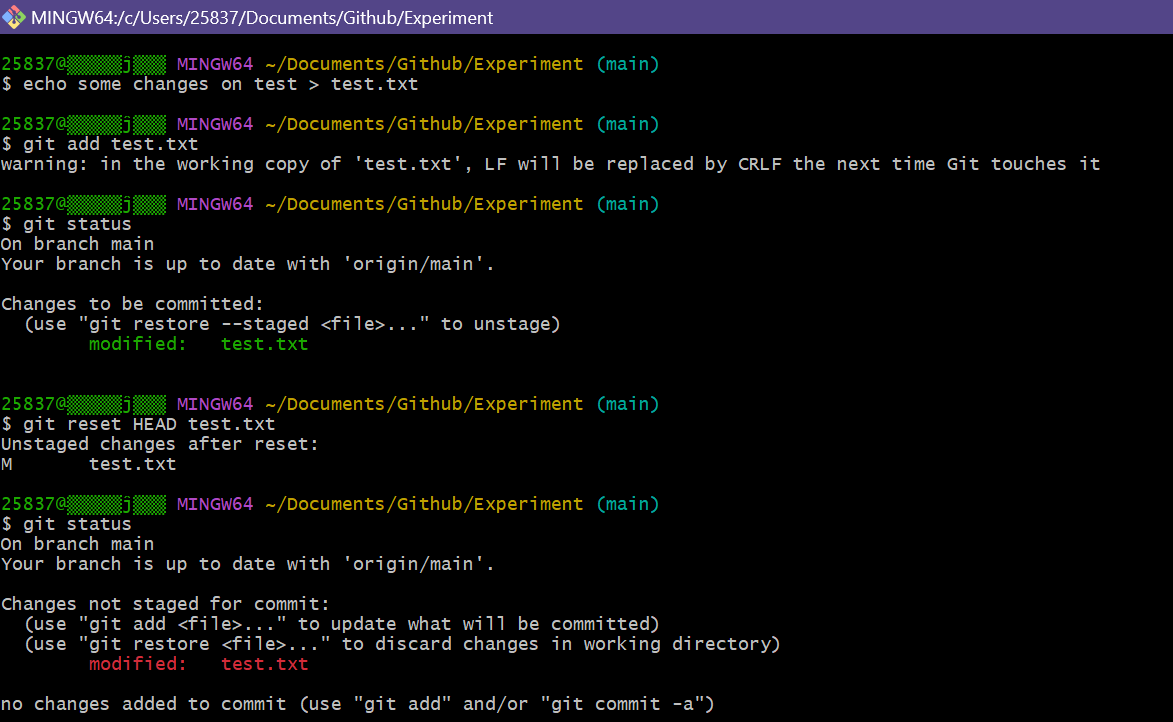
\includegraphics[width=1\textwidth]{im13}
  \caption{操作及结果}
  \label{image-myimage}
\end{figure}

\clearpage

  \subsection{撤销最新一次提交但保留暂存区记录}

将最近的一次commit删除,但是保留这次commit之前的暂存区状态。

相关命令:

\colorbox{lightgray}{\texttt{git reset -- soft HEAD~1}} 删除commit但保留暂存区

\begin{figure}[h!]
  \centering
  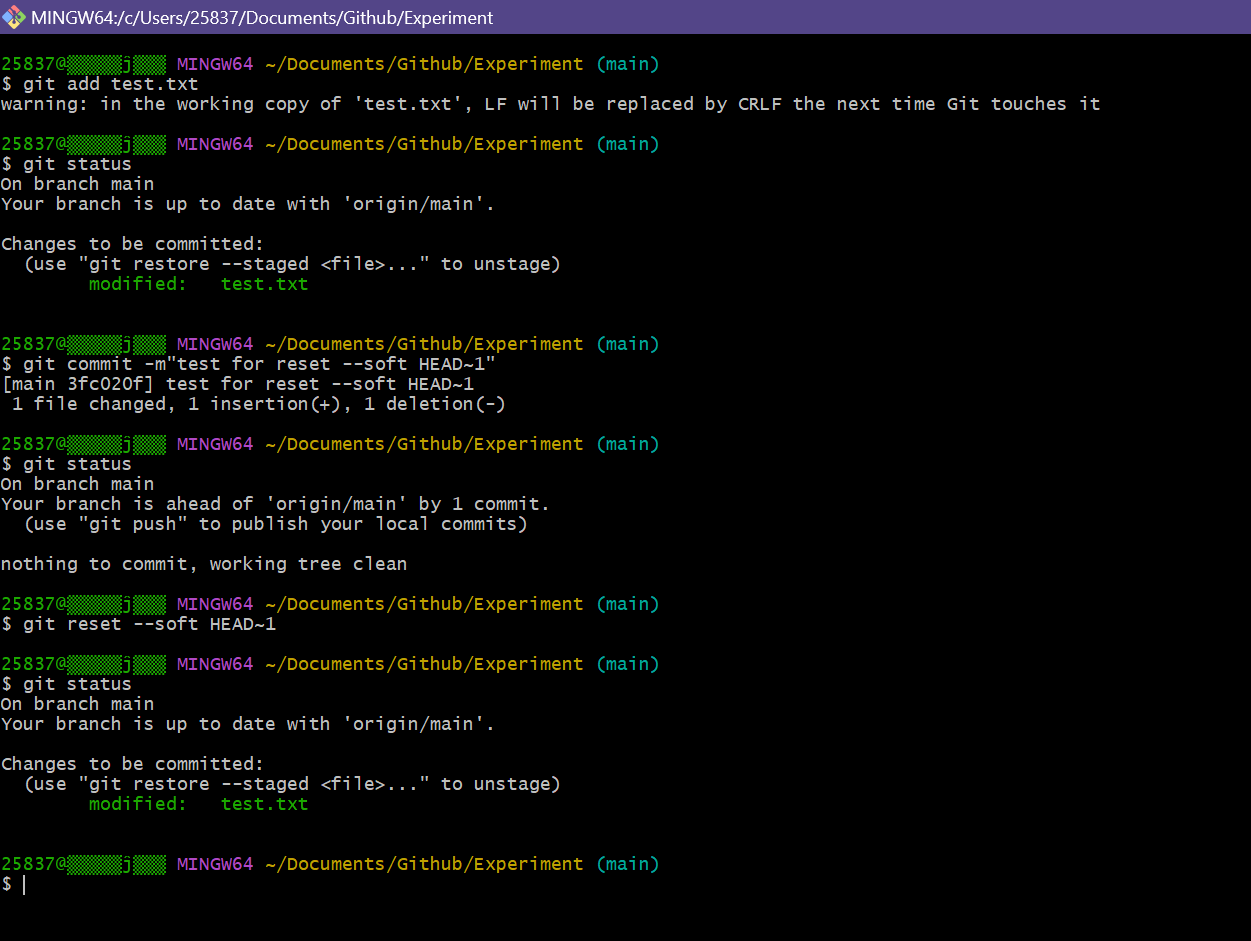
\includegraphics[width=1\textwidth]{im14}
  \caption{操作及结果}
  \label{image-myimage}
\end{figure}

\clearpage

  \subsection{撤销最新一次提交且删除缓存区记录}

将最近一次commit删除,同时删除这次commit之前的暂存区状态。

相关命令:

\colorbox{lightgray}{\texttt{git reset -- hard HEAD~1}} 删除commit同时情况暂存区

\begin{figure}[h!]
  \centering
  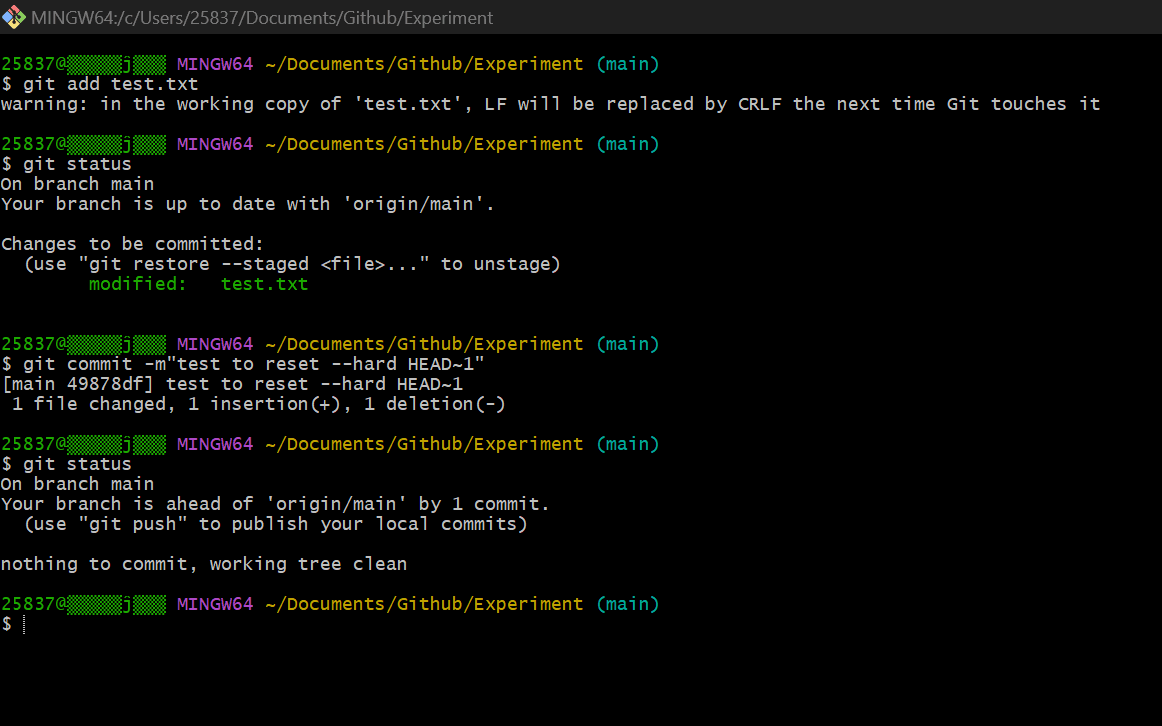
\includegraphics[width=1\textwidth]{im15}
  \caption{操作及结果}
  \label{image-myimage}
\end{figure}

\clearpage

  \section{关于Latex的使用}
  \subsection{文件的基本格式和标题的生成}

每个latex文档,以命令\colorbox{lightgray}{\texttt{\textbackslash documentclass[a4paper, 12pt]\{article\}}}开始,[]是可选的,在里面可以设置你文档的纸张大小和主要字体大小。

紧随上个命令之后可以有一些先导命令,这些命令会影响整个文档。比如我使用命令 \colorbox{lightgray}{\texttt{\textbackslash usepackage\{xcolor\}}} ,引入了可以让我自定义字体色彩的库,同时使用了\colorbox{lightgray}{\texttt{\textbackslash definecolor\{lightgray\}\{RGB\}\{211,211,211\}}},来在全局定义了我用来在展示相关命令和代码时使用的打字机字体后的灰色背景板。

最后,使用\colorbox{lightgray}{\texttt{\textbackslash begin\{document\}}}和\colorbox{lightgray}{\texttt{\textbackslash end\{document\}}} 来包括文档所有的正文部分。

例如:

\begin{verbatim}
\begin{document}
Hello, LaTeX!
\end{document}
\end{verbatim}

关于标题的生成,使用\colorbox{lightgray}{\texttt{\textbackslash title\{这是一个标题\}}}来开始标题生成,\colorbox{lightgray}{\texttt{\textbackslash author\{作者名\}}}来显示作者名,\colorbox{lightgray}{\texttt{\textbackslash date\{相关日期\}}}来显示日期,最后以\colorbox{lightgray}{\texttt{\textbackslash maketitle}}结尾。

例如本篇报告的标题部分代码如下:

\begin{verbatim}
  \title{系统开发工具基础第一次实验报告}
  \author{姓名:杨子程\ 学号:23020007145\ 专业:计算机科学与技术}
  \date{\today}
  \maketitle
\end{verbatim}

%\clearpage

  \subsection{目录的生成}

目录生成的代码较为简单,即\colorbox{lightgray}{\texttt{\textbackslash tableofcontents}}。

例如本篇报告的目录部分代码如下:

\begin{verbatim}
  \tableofcontents
  \newpage %用于开始新的一页,避免目录和正文在同一页
\end{verbatim}

  \subsection{章节的生成}

使用\colorbox{lightgray}{\texttt{\textbackslash chapter\{本章的标题\}}},来生成章;使用\colorbox{lightgray}{\texttt{\textbackslash section\{本节的标题\}}},来生成节;使用\colorbox{lightgray}{\texttt{\textbackslash subsection\{子节的标题\}}},来生成子节。往下还有\colorbox{lightgray}{\texttt{\textbackslash subsubsection\{...\}}}、\colorbox{lightgray}{\texttt{\textbackslash paragraph\{...\}}}、\colorbox{lightgray}{\texttt{\textbackslash subparagraph\{...\}}}等。

例如本篇报告生成章节的部分代码(在没加入正文之前,此subsection往下的部分):

\begin{verbatim}
  \subsection{\color{red}彩色\colorbox{yellow}{\color{green}字体}\color{black}的使用}
  \subsection{自定义页码}
  \subsection{列表(清单)的生成}
  \subsection{表格的生成}
  \subsection{图表的使用}
  \subsection{插入各种数学公式}
  \subsection{书写参考文献}
\end{verbatim}

%\clearpage


  \subsection{\color{red}彩色\colorbox{yellow}{\color{green}字体}\color{black}的使用}

彩色字体的使用要先导入相关的包,例如color、xcolor包。常见的使用彩色字体的命令有\colorbox{lightgray}{\texttt{\textbackslash color\{颜色代码\}正文部分}},其中颜色代码常见的有red、green、blue等等...除此之外还有命令\colorbox{lightgray}{\texttt{\textbackslash clorbox\{颜色代码\}{正文部分}}},彩色背景板等...colorx中提供自定义颜色的命令\colorbox{lightgray}{\texttt{\textbackslash definecolor\{lightgray\}\{RGB\}\{211,211,211\}}},例如这串代码自定义颜色为浅灰色。

本小节标题颜色的代码为:

\begin{verbatim}
  \color{red}彩色\colorbox{yellow}{\color{green}字体}\color{black}的使用
\end{verbatim}

%\clearpage

  \subsection{自定义页码}

我学习到的自定义页码可以使用包fancyhdr,其中提供了一些改变默认页码表示,自定义页码表示的方法。下面展示本篇报告中关于取消正下方中间显示页码,改为下方右侧显示页码的操作。

\begin{verbatim}
  \usepackage{fancyhdr}  % 引入 fancyhdr 宏包
  \pagestyle{fancy}      % 使用 fancyhdr 提供的页面样式
  \fancyhf             % 清除默认设置
  \fancyfoot[R]{\thepage} % 将页码放在右下角
%以上操作都是针对整个文档进行的所以放在\begin{document}之前
\end{verbatim}

%\clearpage

  \subsection{列表(清单)的生成}

使用\colorbox{lightgray}{\texttt{\textbackslash begin\{enumerate\}}}和\colorbox{lightgray}{\texttt{\textbackslash end\{enumerate\}}}作为一对,来开始与结束一个有序列表,对应将enumerate换为itemize使用无序列表,列表有些类似清单的感觉。在begin和end中间使用\colorbox{lightgray}{\texttt{\textbackslash item 项目名称}}来表示清单中的各项

下面展示一个我写的列表,安排我一天的任务

\begin{enumerate}
  \item 学习数学建模

  \item 完成系统开发基础工具的实验报告
    \begin{itemize}
      \item Git部分

      \item Latex部分
    \end{itemize}

  \item 完成计算机工程伦理的课程报告

  \item 取快递
    \begin{itemize}
      \item 数据线

      \item 眼罩
    \end{itemize}
\end{enumerate}

以下是相关代码

\begin{verbatim}
  \begin{enumerate}
  \item 学习数学建模

  \item 完成系统开发基础工具的实验报告
    \begin{itemize}
      \item Git部分

      \item Latex部分
    \end{itemize}

  \item 完成计算机工程伦理的课程报告

  \item 取快递
    \begin{itemize}
      \item 数据线

      \item 眼罩
    \end{itemize}
\end{enumerate}
\end{verbatim}

  \subsection{表格的生成}

使用\colorbox{lightgray}{\texttt{\textbackslash begin\{tabular\}\{...\}}}和\colorbox{lightgray}{\texttt{\textbackslash end\{tabular\}}}作为一对来生成表格。其中begin后的...部分由指定列相关内容的代码取代。涉及有\colorbox{lightgray}{\texttt{l,r,c}}分别表示每列的对齐方式(左、右、中),还有\colorbox{lightgray}{\texttt{|}},来表示分割列。在begin之后还可输入的有:\colorbox{lightgray}{\texttt{\&,\textbackslash \textbackslash,\textbackslash hline,\textbackslash cline\{...\}}},分别表示分割列(与前面提到分割不同的是,前面是文档显示的分割,此处是代码逻辑的分割,因为\&将会处于不同列的正文之间);换行;分割行;分割指定行(...处为指定方法,常见的指定为\colorbox{lightgray}{\texttt{列1的序号-列2的序号}},这样会添加一个分割行的线,从列1贯穿到列2)

例如,以下是我完成的参考资料上提供的实践题表格:

\begin{tabular}{l|ccc}
   & Year  \\
  \cline{2-4}
  City & 2006 & 2007 & 2008    \\
  \hline
  London & 45789 & 46551 & 51298 \\
  Berlin & 34549 & 32543 & 29870 \\
  Paris & 49835 & 51009 & 51970
\end{tabular}
\\

以下是上图的代码:

\begin{verbatim}
\begin{tabular}{l|ccc}
   & Year  \\
  \cline{2-4}
  City & 2006 & 2007 & 2008    \\
  \hline
  London & 45789 & 46551 & 51298 \\
  Berlin & 34549 & 32543 & 29870 \\
  Paris & 49835 & 51009 & 51970
\end{tabular}
\end{verbatim}

  \subsection{图表的使用}

图表插入要用到包graphicx,例如在我本篇报告的第一个实验插入的第一张图片,使用了如下代码:

\begin{verbatim}
\begin{figure}[h]
  \centering
  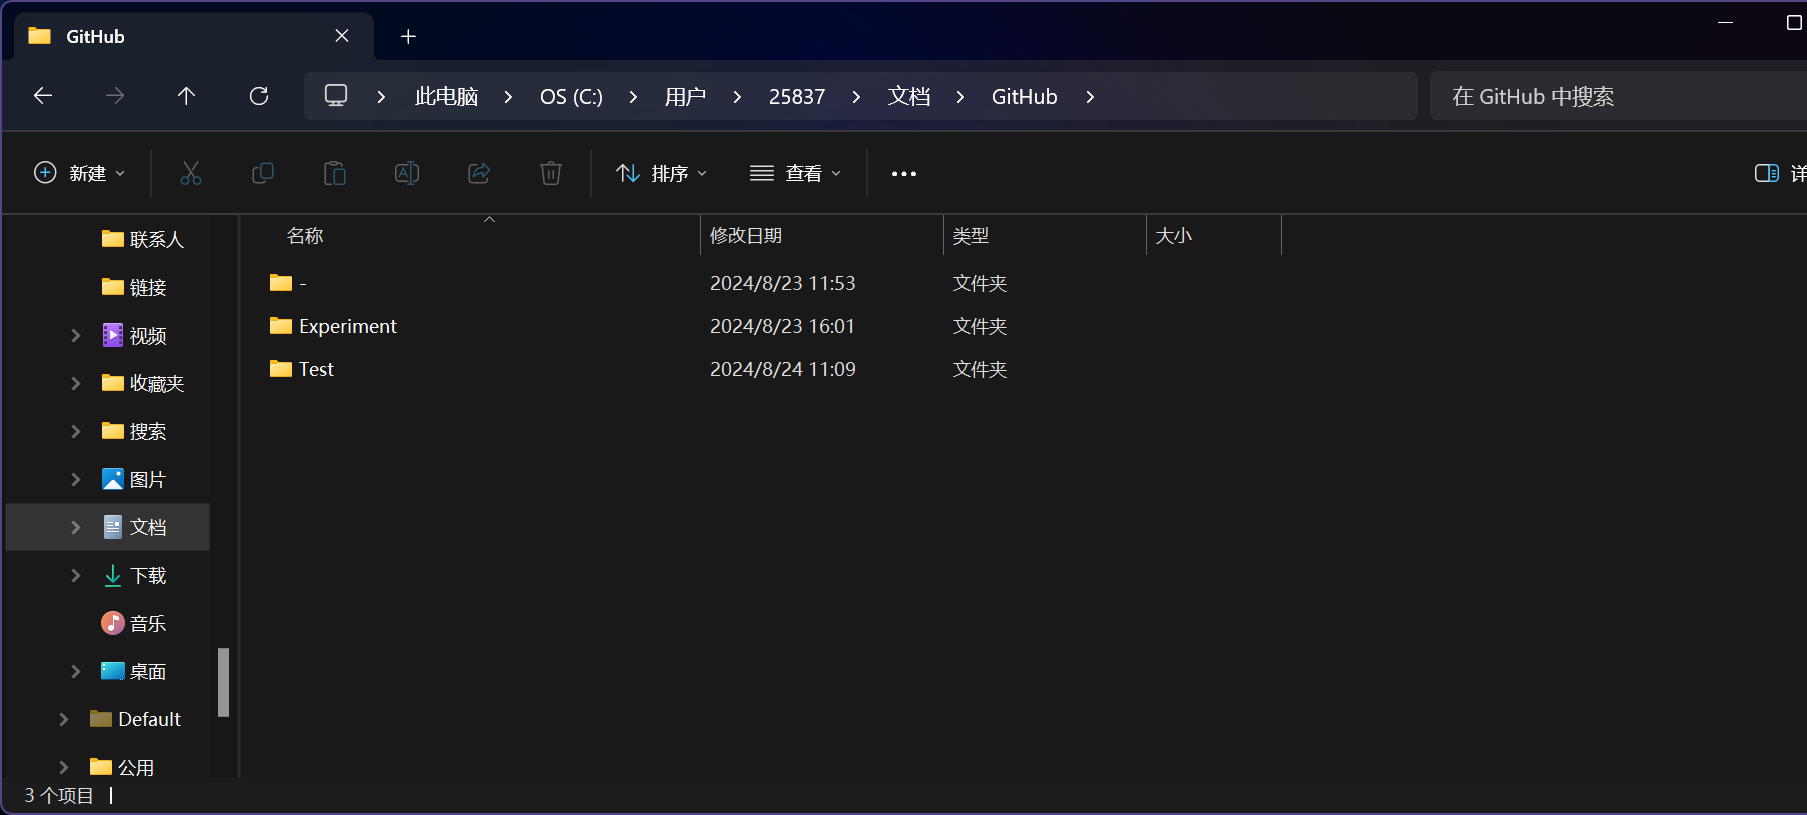
\includegraphics[width=1\textwidth]{im1}
  \caption{本地文件夹}
  \label{image-myimage}
\end{figure}
\end{verbatim}

其中涉及到\colorbox{lightgray}{\texttt{\textbackslash centering}},表示插入图片的位置,centering表示居中。对于\colorbox{lightgray}{\texttt{\textbackslash includegraphic[]\{\}}},[]是可选的,用于设置图片的大小尺寸、大括号中包括了图片的地址,当图片与latex文档在同一文件夹下时只需要文件名即可\colorbox{lightgray}{\texttt{\textbackslash caption\{\}}}用于设置图片名,大括号中书写。最后使用label添加了一个标签,这是可选的。以上提到的都要插入\colorbox{lightgray}{\texttt{\textbackslash begin\{figure\}}}和\colorbox{lightgray}{\texttt{\textbackslash end\{figure\}}}对之间,这对代码表示要开始插入图片。

  \subsection{插入各种数学公式}

数学公式的插入使用\colorbox{lightgray}{\texttt{\$ \$}}或\colorbox{lightgray}{\texttt{\$\$ \$\$}}进行标记。常见的命令有,表示上下标的\colorbox{lightgray}{\texttt{\^}}和\colorbox{lightgray}{\texttt{\_}};表示分数的\colorbox{lightgray}{\texttt{\textbackslash frac{分子}{分母}}};表示根号的\colorbox{lightgray}{\texttt{\textbackslash sqrt{...}}};表示求和的\colorbox{lightgray}{\texttt{\textbackslash sum}};表示积分的\colorbox{lightgray}{\texttt{\textbackslash int}}等等的数学公式

下面是我就参考资料的实践题进行的实现:

\begin{align}
  e &= mc^2 \\
  \pi &= \frac{c}{d} \\
  \frac{d}{dx}e^x &= e^x  \\
  \frac{d}{dx}\int_0^\infty f(s)ds & = f(x) \\
  f(x) & = \sum_i 0^\infty \frac{f^(i)(0)}{i!}x^i \\
  x & = \sqrt{\frac{x_i}{z}y}
\end{align}

以下是上面公式的代码:

\begin{verbatim}
\begin{align}
  e &= mc^2 \\
  \pi &= \frac{c}{d} \\
  \frac{d}{dx}e^x &= e^x  \\
  \frac{d}{dx}\int_0^\infty f(s)ds & = f(x) \\
  f(x) & = \sum_i 0^\infty \frac{f^(i)(0)}{i!}x^i \\
  x & = \sqrt{\frac{x_i}{z}y}
\end{align}
\end{verbatim}

  \subsection{书写参考文献}

我在按照参考网站引用参考文献的时候发生错误,经上网查阅发现是因为我的这份latex文档名字中包含了中文字符(非ASCII字符),导致一些辅助文件例如.aux文件也含有这些字符,从而导致了编译失败。下面是我新建了一个latex文档,书写的有关参考文献的内容:

\begin{figure}[h!]
  \centering
  
\includegraphics[width=1\textwidth]{im16}
  \caption{如上}
  \label{image-myimage}
\end{figure}

相关代码:

\begin{verbatim}
\bibliographystyle{plain}
\bibliography{MyReference}
\end{verbatim}

第一行说明了引用文献时的排版样式,第二个MyReference是当前目录下的bib文件名,书写参考文献用的文件。注意,在有参考文献的时候,要先执行BibTex编译,再使用正常的pdfLaTex编译,这样才会得到正确的结果。

\end{document}